\documentclass[a4paper, xelatex, ja=standard]{bxjsarticle}
\setpagelayout*{top=25truemm,bottom=25truemm,left=25truemm,right=25truemm}

% パッケージインストール
\usepackage{plisting}
\usepackage{docmute}

% 文書開始
\begin{document}

\section{問題設定}
被乗数と乗数の2つの整数を端末から入力し,
その積を出力するプログラムを作成する.

\begin{lstlisting}[caption=例,label=]
[onosans@onosans-shyvana w02]$ ./ex.out
被乗数と乗数を入力してください
被乗数: 365
乗数: 17
365 x 17 = 6205
\end{lstlisting}

\section{問題分析}
今回の問題はまずユーザーに対しどのような値が欲しいのか示す必要がある.
そのため\texttt{printf}で「被乗数と乗数を入力してください」と出力する.

次に乗数, 被乗数の入力を受け付ける.
まず入力された値を一度メモリに保存する必要があるため
整数(int)型の変数を2つ宣言する.
次にどちらの値を受け付けるかなどの細かい表示をして,
\texttt{scanf}を使い先ほど宣言した変数に入力された値を代入する.

最後にそれらを計算した結果を出力すれば終了となる.


\section{設計}
今回作成するプログラムのフローチャートを以下に示す.

\begin{figure}[h]
\centering
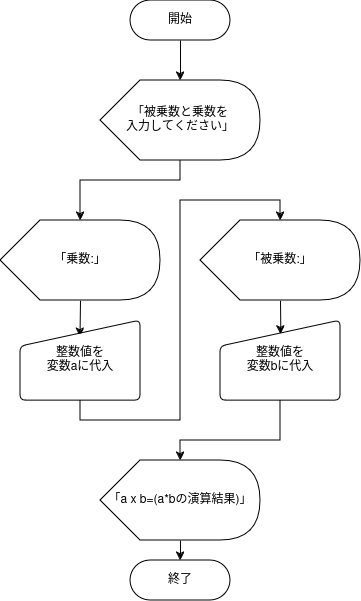
\includegraphics[scale=0.5]{../img/flowchart.drawio.png}
\caption{フローチャート}
\label{}
\end{figure}

\section{実装}
まず変数表を以下に載せる.

\begin{table}[h]
\centering
\caption{変数表}
\label{}
\begin{tabular}{|c|c|c|c|}
\hline
データ & 変数名                         & データ型 & 説明  \\ \hline
入力  & \texttt{a} & int  & 被乗数 \\ \hline
入力  & \texttt{b} & int  & 乗数  \\ \hline
\end{tabular}
\end{table}

それぞれの変数の役割は載せた表の通りである.
次に今回書いたコードを載せる.

\begin{lstlisting}[caption=ソースコード,label=s01]
#include <stdio.h>

int main(void){
	int a, b; // 整数型の変数a, bを宣言
	printf("被乗数と乗数を入力して下さい\n");
	printf("被乗数:");
	scanf("%d", &a); // aに入力された値を代入
	printf("乗数:");
	scanf("%d", &b); // bに入力された値を代入

	// 乗算した結果の出力
	printf("%d x %d = %d\n", a, b, a*b);

	return 0;
}
\end{lstlisting}

前回から使っているものの説明は省く.
\texttt{scanf}関数はターミナルからの入力を受け付ける関数である.
入力された値をどこの変数にどのような形式で保存するのかを,
第1引数に書式指定子, 第2引数に変数のメモリ上のアドレスを渡すことで
指定の変数に値を保存している.
10進数の場合, 書式指定子は\texttt{\%d},
変数のアドレスは変数名の前に\texttt{\&}をつける.

次に\texttt{printf}の新しい使い方として書式指定子を用いて
変数の値を代入する方法がある.
使い方はソースコード\ref{s01}のように
対応する場所に書式指定子を入れ,
対応する値(変数や演算)をコンマ区切りで入れていく.

これらの機能を使って以上のようにコードを組み立てた.

\section{検証}
実行結果は以下の通りである.

\begin{figure}[h]
\centering
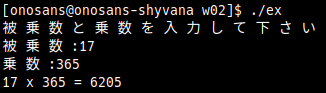
\includegraphics[scale=1.0]{../img/terminal_result.png}
\caption{実行結果}
\label{}
\end{figure}

実行環境は前回と異なり, 
ChromeBookにArchLinuxを入れたもので実行した.

\section{考察}
\subsection{オーバーフローさせてみる}
私の使用しているものも
\texttt{int}型のサイズは32bitのため
-2147483648から2147483647までの整数を表現することができる.
試しに2147483648と1を入力してみる.
すると結果は以下のようになる.
\begin{lstlisting}[caption=オーバーフロー1,label=]
[onosans@onosans-shyvana w02]$ ./ex.out
被乗数と乗数を入力してください
被乗数: 2147483648
乗数: 1
2147483648 x 1 = -2147483648
\end{lstlisting}

\begin{table}[h]
  \centering
  \caption{}
  \label{}
  \begin{tabular}{|c||c|c|}
  \hline
  & 10進数 & 2進数 \\ \hline
  被乗数 & 2147483648 & 1000 0000 0000 0000 0000 0000 0000 0000 \\ \hline
  答え & -2147483648(2の補数) & 1000 0000 0000 0000 0000 0000 0000 0000 \\ \hline
  \end{tabular}
\end{table}
このように2進数で見ても正しいことがわかる.
2の補数の仕組み上,
表現できる最大値の次の値は表現できる最小値になることを
改めて確認することができた.

% このバグを改善する方法としては
% パワープレイであれば使うbit数を増やせば良いが,
% 少し工夫をするのであれ

\subsection{乗算を使わない実装}
この授業とは関係ないが計算機アーキテクチャで
「掛け算は足し算の繰り返しで実装できる」
ということを聞いたので,
足し算を繰り返すver.を作ってみた.
尚, 繰り返しの記述方法は既に知っていたので
参考文献には記述していない.
\begin{lstlisting}[caption=加算のみでの実装,label=]
#include <stdio.h>

int main(void){
	int a, b;
	printf("被乗数と乗数を入力して下さい\n");
	printf("被乗数:");
	scanf("%d", &a);
	printf("乗数:");
	scanf("%d", &b);

	int ans=0; // 積を保持する変数

	// b回繰り返し実行するという意味
	for(int i=0; i < b; i++){
		ans+=a; // ansにaの値を加算する
	}

	// 乗算した結果の出力
	printf("%d x %d = %d\n", a, b, ans);

	return 0;
}
\end{lstlisting}

\begin{table}[h]
\centering
\caption{変数表2}
\label{}
\begin{tabular}{|c|c|c|c|}
\hline
データ & 変数名 & データ型 & 説明  \\ \hline
出力 & \texttt{num} & int  & 演算途中の値の保存 \\ \hline
入力 & \texttt{a} & int  & 被乗数 \\ \hline
入力 & \texttt{b} & int  & 乗数  \\ \hline
\end{tabular}
\end{table}
こちらは乗数の回数分だけ加算を繰り返しているだけである.
今回の場合整数型なのでこれで実装することができているが,
浮動小数点型になった場合は1以下の部分については
被乗数を割れば実装できそうだがそもそも割り算をどう実装するのか
あまり思いついていない状況ではある.

\subsection{乗算も繰り返しも使わない実装}
繰り返しでは実行が遅くなってしまってとても良くない
(そもそもハードに搭載されているものが最適化されているので
一番最初の実行方法が最速だと思われるが)
のでプログラム上で乗算器を再現してみる.



\section{所感}

\begin{thebibliography}{9}
\bibitem{key1} 乗算器, \url{https://ja.wikipedia.org/wiki/%E4%B9%97%E7%AE%97%E5%99%A8}.
\bibitem{key2} 符号拡張, \url{https://ja.wikipedia.org/wiki/%E7%AC%A6%E5%8F%B7%E6%8B%A1%E5%BC%B5}
\end{thebibliography}

\end{document}